\documentclass[10pt,oneside,english,a4paper]{article}

\usepackage[english]{babel}
\usepackage[IL2]{fontenc}
\usepackage[utf8]{inputenc}
\usepackage{graphicx}
\usepackage{url}
\usepackage{hyperref} 

\usepackage{cite}

\pagestyle{headings}

\title{Usage of deep learning techniques, super-resolution and upscaling in video games\thanks{Semester project in the subject Methods of engineering work (MIP), academic year 2022/23, supervising teacher: Ing. Igor Stupavský}}

\author{Teodor Reménység\\[2pt]
	{\small Slovenská technická univerzita v Bratislave}\\
	{\small Fakulta informatiky a informačných technológií}\\
	{\small \texttt{xremenyseg@stuba.sk}}
	}

\date{\small 6. November 2022}



\begin{document}

\maketitle

\begin{abstract}
The main goal of this paper is to enlighten the reader with the current technologies used in video games, which work to lessen the workload on the processing units of the user’s computer during rendering and therefore enhance their immersion and overall experience while playing. Further, it will look at the other possible applications of these technologies and explore where and how they are currently being used, their positives, negatives and will showcase some of their teething troubles and cases where they shouldn’t have been used. A conclusion will be drawn on whether or not these technologies can and should be massively adopted based on the approaches that are possible today.
\end{abstract}



\section{Introduction}

Recently, video games have begun to look more and more realistic. Even when compared to games from the early 2010s, the difference in graphics quality is very noticeable. This exponential improvement in quality can largely be attributed to the improvement of graphical processing unit (GPU) hardware. However, at this point in time, it seems as though the latest improvements in hardware have come at great expense in the aspects of power consumption and size. A different way to further improve graphical quality is through the use of software. This paper will explore such software solutions, mainly in respect to current technologies that were developed for use in video games.

The problem of increasing GPU workloads is further elaborated upon in the second section (section~\ref{rise}), then, in the third (section~\ref{aasr}) and fourth (section~\ref{deep}) sections, this paper describes some individual types of the beforementioned software solutions, what each of them offer and how they compare. In the fifth section (section~\ref{challenges}), this paper expands on the current challenges of said solutions and the potential methods for overcoming the challenges. Finally, a conclusion (section~\ref{conclusion}) is given at the end on the current state of graphical processing in video games, the solutions to problems arising therein and their potential future developments.


\section{Rising GPU workloads} \label{rise}

As can be seen from fig.~\ref{f:graph}, GPU hardware capabilities have grown exponentially in recent years. However, the demand for these capabilities has also increased exponentially, especially in regards to real-time rendering (RTR). RTR is "the generation of multiple high-resolution frames every second in real time, to give the illusion of motion and interaction. RTR for modern desktop, VR and mobile device applications is becoming exponentially difficult because of higher resolutions and a general focus on photorealism at high framerates. Recent high-end monitors now provide support for resolutions up to 7680 x 4320 pixels at refresh rates of 240 Hz. This, along with recent advances and implementations of physical shading, ray tracing, accurate physics simulations, and higher quality texture models, makes it difficult for even current generation GPUs to render images at native resolutions without compromising framerates."\cite{9441822}

\begin{figure*}[tbh]
\centering
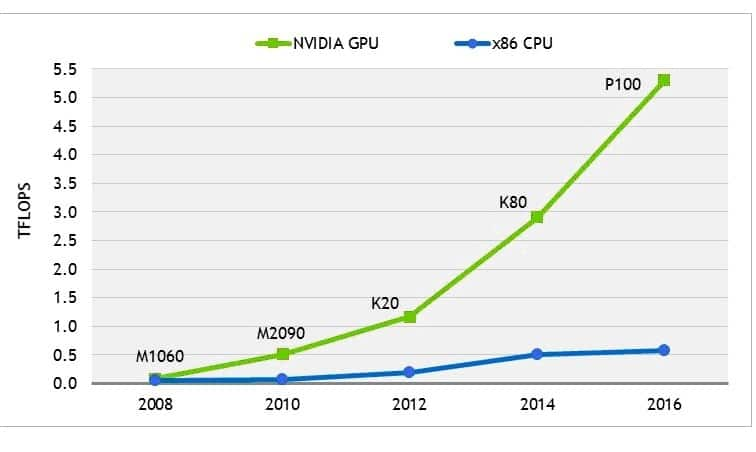
\includegraphics[scale=0.4]{gpugraph.jpg}
\caption{The evolution of GPU performance.}
\url{https://www.rtinsights.com/gpus-the-key-to-cognitive-computing/}
\label{f:graph}
\end{figure*}



\section{Anti-aliasing and Superresolution} \label{aasr}

\subsection{Anti-aliasing} \label{aasr:aa}

\subsection{Superresolution} \label{aasr:sr}

\section{Deep Learned Technologies} \label{deep}

\subsection{Deep Learning Super Sampling} \label{deep:dlss}

\subsection{Neural Super Sampling} \label{deep:neural}

\section{Challenges and potential solutions} \label{challenges}




\section{Conclusion} \label{conclusion}


%\acknowledgement{\ldots}



\bibliography{literatura}
\bibliographystyle{plain}
\end{document}
